\textbf{مورد استفاده:}
درخواست پروژه
\\
\textbf{شرح مختصر :UC}
در این قسمت فریلنسر پیشنهادات خود برای انجام پروژه را برای کارفرما ارسال می‌کند.
\\
\textbf{پيش شرط:}
ورود به داشبورد فریلنسر
\\
\textbf{سناريو اصلی:}
\begin{enumerate}
\item
شروع
\item
فریلنسر دکمه درخواست پروژه را انتخاب می‌کند و سیستم فرم خام پیشنهاد به کارفرما را نمایش می‌دهد
\item
فریلنسر فرم را تکمیل می‌کند و با دکمه ارسال، اطلاعات را به سیستم ارسال می‌کند.
\item
سیستم اطلاعات را بررسی می‌کند و در بانک اطلاعات ثبت می‌کند.
\item
پایان
\end{enumerate}

\noindent
\textbf{پس شرط:}
کارفرما باید درخواست فریلنسر را تایید کند.
\\
\textbf{سناريوهای فرعی:}
\\
\textbf{سناريو فرعی 1:}
خطا در اطلاعات فرم درخواست پروژه
\\
\textbf{شرح مختصر :UC}
این سناریو در مرحله ۴ سناریو اصلی در صورت خطا در اطلاعات فرم اجرا می‌شود.
\begin{enumerate}
\item
شروع
\item
اطلاعات فرم بررسی می‌شود و خطاها مشخص می‌شوند.
\item
یک پیغام به فریلنسر نمایش داده می‌شود و درخواست اصلاح اطلاعات فرم را دارد.
\item
از مرحله 3 سناریو اصلی ادامه پیدا می‌کند.
\item
پایان
\end{enumerate}

\noindent
\textbf{سناريو فرعی 2:}
درخواست با موفقیت ثبت شود
\\
\textbf{شرح مختصر :UC}
این سناریو در مرحله ۴ سناریو اصلی در صورت موفقیت آمیز بودن ثبت درخواست پروژه اجرا می‌شود.
\begin{enumerate}
\item
شروع
\item
اطلاعات فرم بررسی می‌شود و یک پیغام به فریلنسر نمایش داده می‌شود که اطلاعات با موفقیت ثبت شده است.
\item
از مرحله 4 سناریو اصلی ادامه پیدا می‌کند.
\item
پایان
\end{enumerate}

\noindent
\textbf{پس شرط:}
ندارد.




\begin{figure}[H]
	\includegraphics[width=0.7\textwidth]{Diagram/2.Activity/داشبورد-کاربر/فریلنسر/درخواست-پروژه.jpg}
	\centering
	\caption{دیاگرام فعالیت درخواست پروژه}
	\label{fig:a:درخواست-پروژه}
\end{figure}
\begin{figure}[H]
	\includegraphics[width=1\textwidth]{Diagram/3.Sequence/داشبورد-کاربر/فریلنسر/درخواست-پروژه.jpg}
	\caption{دیاگرام توالی درخواست پروژه}
	\centering
	\label{fig:s:درخواست-پروژه}
\end{figure}
\begin{figure}[H]
	\includegraphics[width=1\textwidth]{Diagram/4.Collaboration/داشبورد-کاربر/فریلنسر/درخواست-پروژه.jpg}
	\centering
	\caption{دیاگرام همکار درخواست پروژه}
	\label{fig:c:درخواست-پروژه}
\end{figure}